\section{An Infinite Hierarchy of Prezero Points}

Now that we have visually demonstrated the existence of these two ``primary sequences'' of parameter values, we will introduce some results which add an infinite hierarchy of complexity in between each parameter value in the aforementioned sequences. This result is best summarized by Proposition \ref{mainprop}:

\begin{customthm}{\ref{mainprop}}
	Suppose we have two distinct parameter values $z_{n_1}^{C\alpha0}, z_{n_2}^{C\beta0} \in (\pl, \pr)$ where $\alpha$ and $\beta$ are coding sequences such that $\alpha_i \neq \beta_i$ for at least one $i$. Then there must be at least one other prezero parameter value $z_{n_3}^{C\gamma0}$ on the interval $\inte{z_{n_1}^{C\alpha0}}{z_{n_2}^{C\beta0}}$ such that $\alpha_i \neq \gamma_i$ and $\beta_j \neq \gamma_j$ for at least one $i$ and one $j$.
\end{customthm}

% \begin{figure}[h]
% \centering
% 	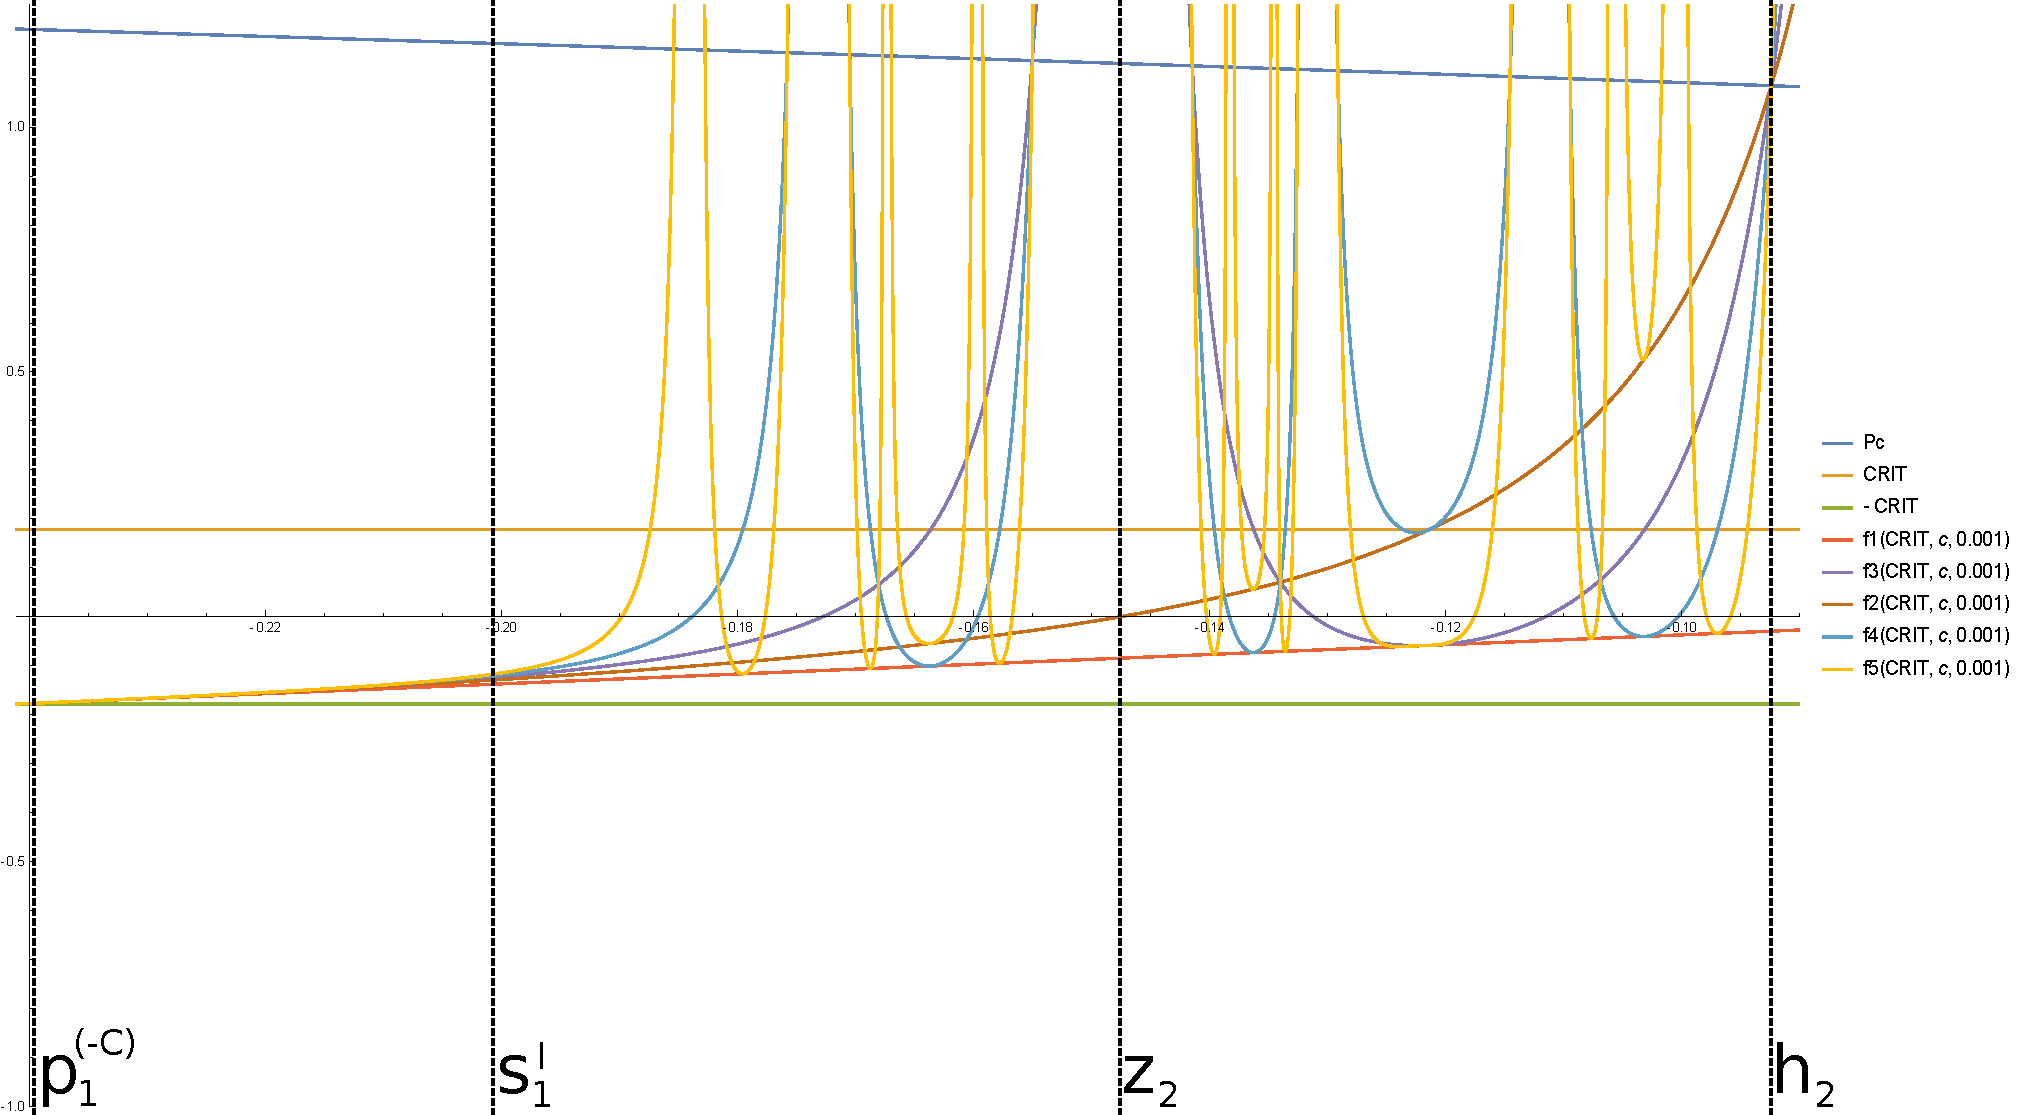
\includegraphics[width=.75\textwidth]{./img/cplot.pdf}
% 	\caption{Plot of the first five iterates of $C$ with respect to $c$}
% 	\label{cplot}
% \end{figure}

In this section we will briefly provide some discussion and figures which provide some intuition as to what this proposition means. First consider the plot of the first 3 iterates of the right hand critical point with respect to $c$ as shown in the Figure \ref{hqcplot}. This plot is a useful visual guide because we can quickly see how the behavior of lower iterates affects the behavior of higher iterates. One of the most notable behaviors that can be observed is how some $n^{th}$ iterate mapping to zero forces all higher iterates to be $\infty$, a fact easily proven as Lemma \ref{zero}. Additionally, we note that for all $n > 2$, $f^n_{\pr} (C) = P_c$ and $f^n_{\pl} (C) = -C$ as discussed in the introductory remarks. Thus at either end of this interval, all iterates are clamped to some specific value, regardless of the behavior in between.

To provide an example of what Proposition \ref{mainprop} is saying, we will provide a sample case from the proof of Proposition 4.2. Figure \ref{fig:case1} shows the first case where we have some parameter $z_3^{CrF0}$ to the left and some parameter $z_4^{CrFL0}$ to the right. This proposition forces the existence of some other $z_{n_1}$ between these two parameter values. Two satisfactory parameter values are labeled as $z_5^{CrFLF0}$ and $z_5^{CrFLL0}$. Note that these values were found by looking at $f^4_c (C)$ which has a parameter value $p_4^{CrFL}$ in between $z_3^{CrF0}$ and $z_4^{CrFL0}$. Then we show in Chapter 4 that $f^1_c (C) < 0$ for $c \in (\pl, \pr)$, meaning that when we look at the fifth iterate at this parameter value we get:
\[
	f^5_{p_4^{CrFLC}} (C) = f_{p_4^{CrFLC}}\left (f^4_{p_4^{CrFLC}} (C)\right) = f_{p_4^{CrFLC}} (C) < 0
\]
Thus we have a $c$ value for which $f^5_c (C) < 0$ and two points where the fifth iterate must be $\infty$ (at $z_3^{CrF0}$ and $z_4^{CrFL0}$) so in between there must be two points where the fifth iterate is 0, these being $z_5^{CrFLF0}$ and $z_5^{CrFLL0}$. 
\begin{figure}
	\centering
	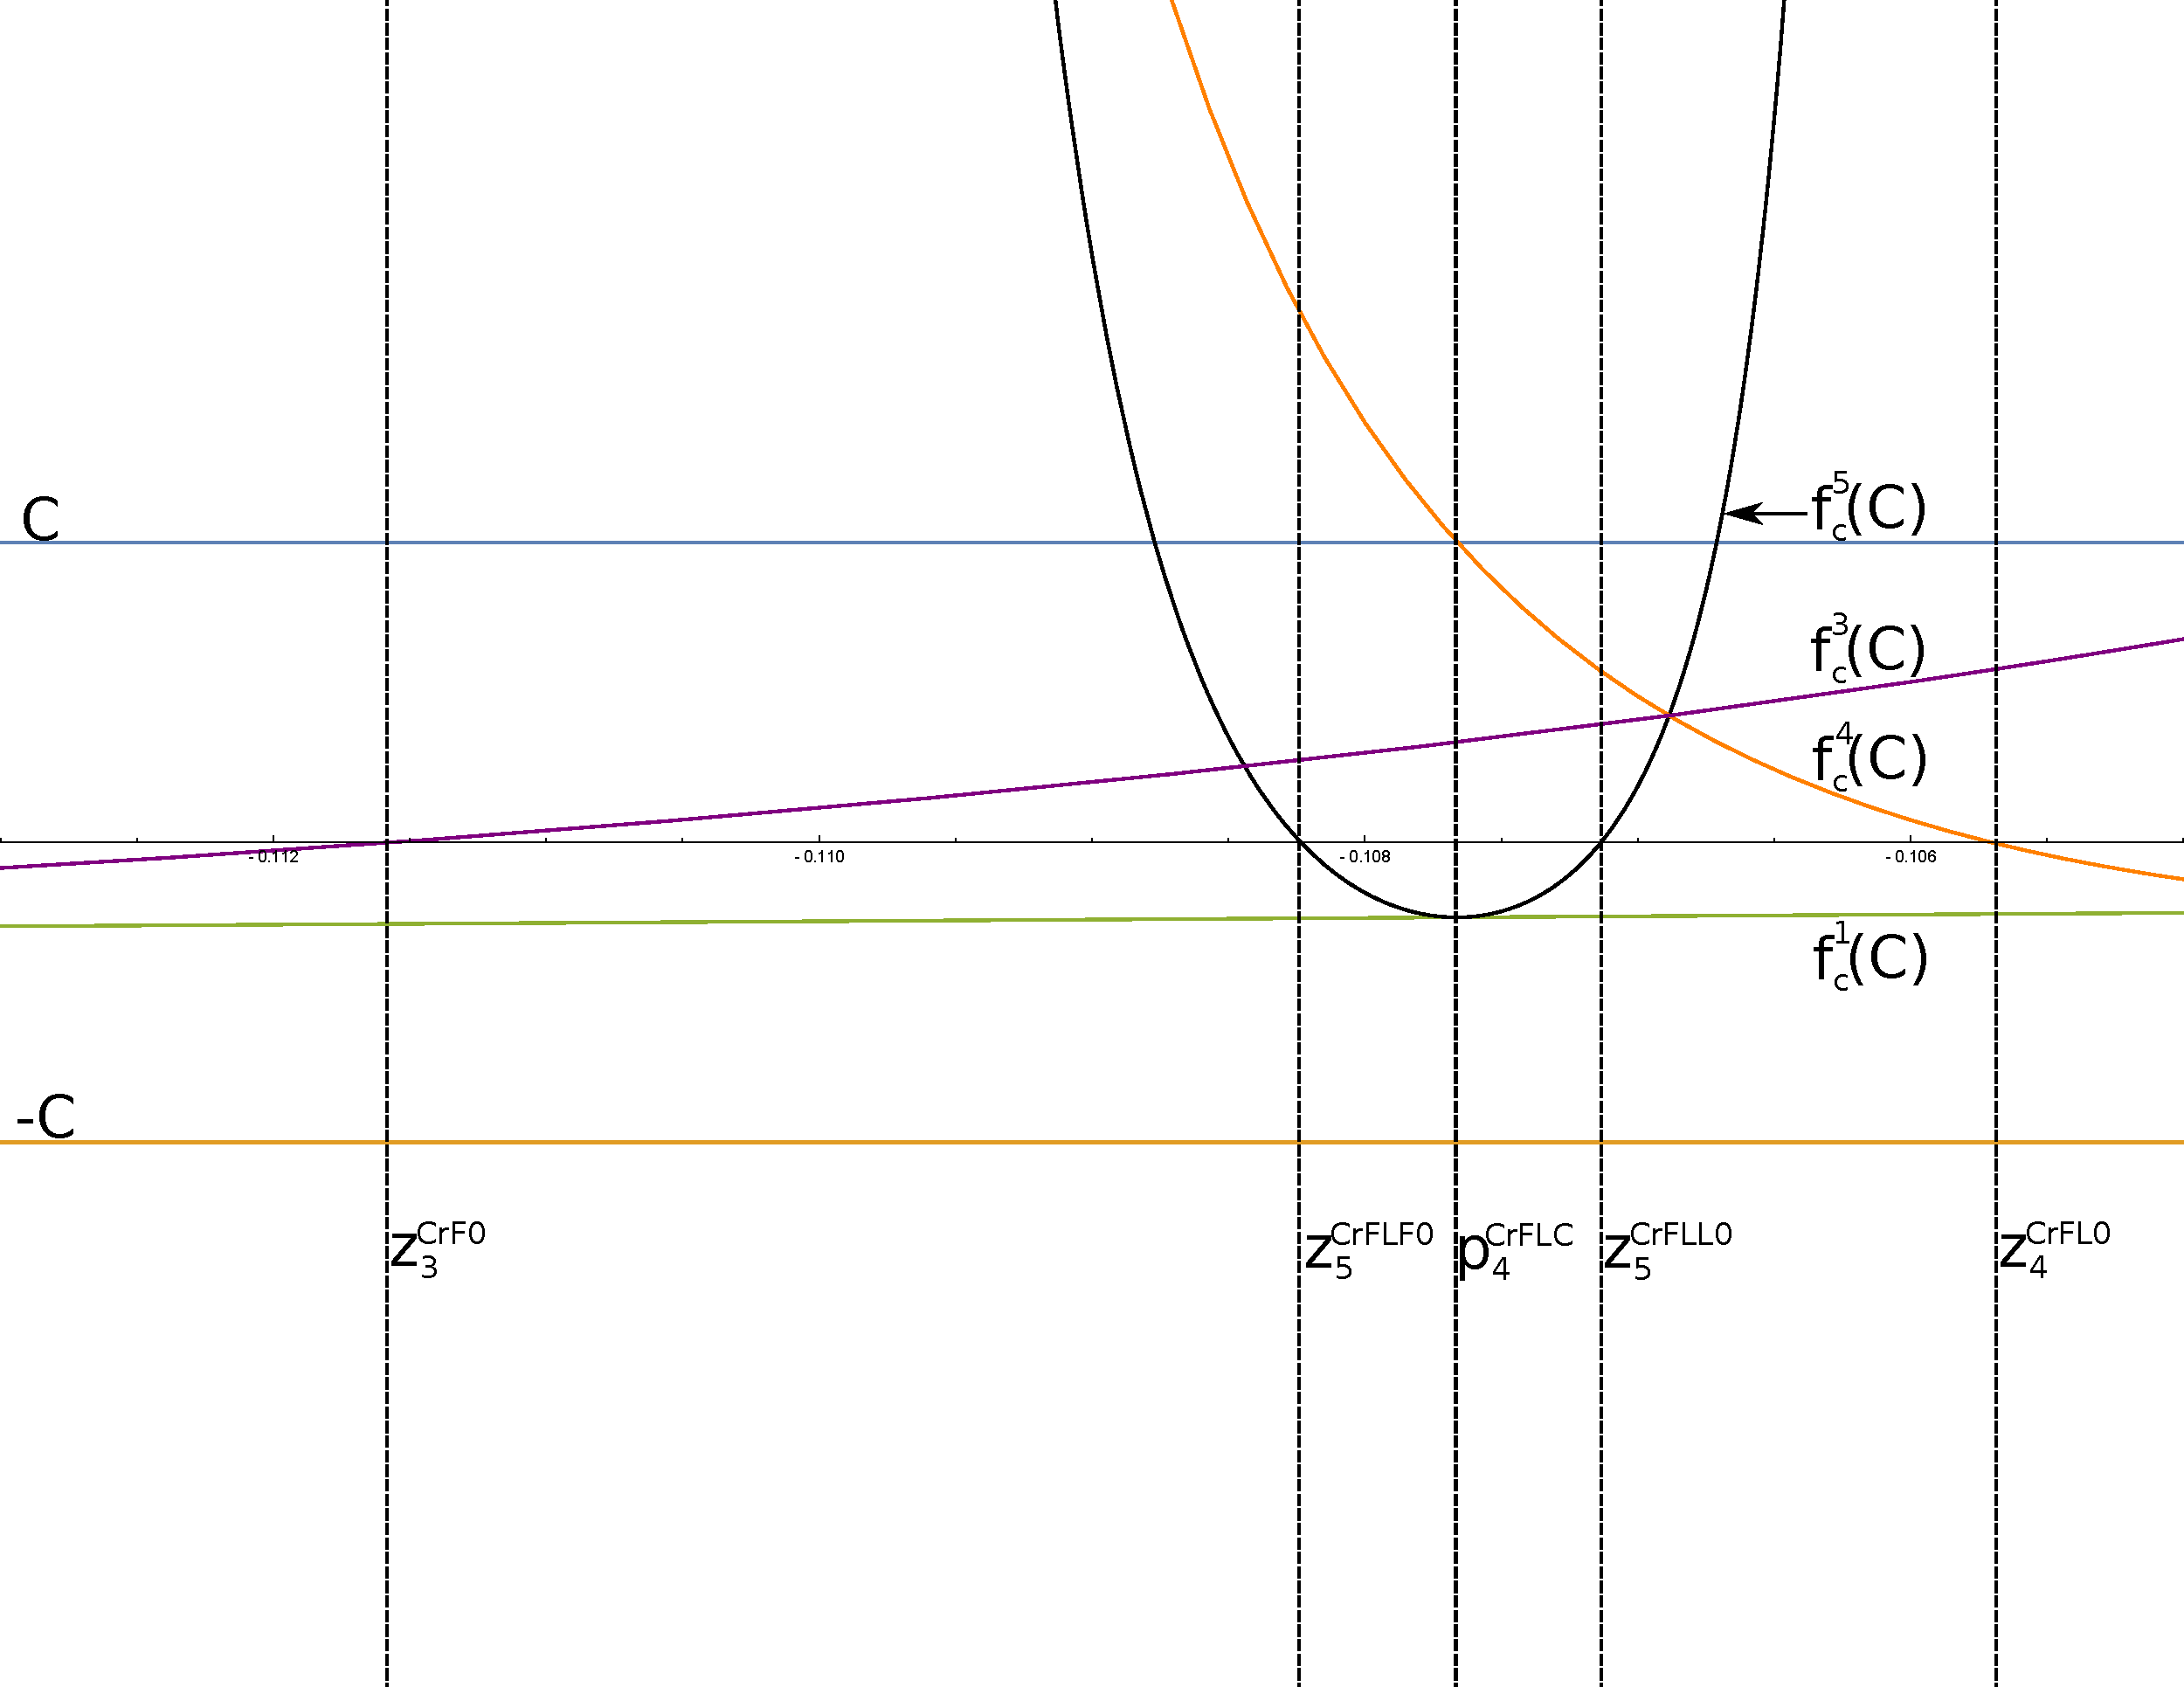
\includegraphics[width=.75\textwidth]{./img/pre0case1p}
	\caption{Plot of $f_c (C),f^3_c (C),f^4_c (C)$ and part of $f^5_c (C)$ showing the existance of two prezero parameter values $z_5^{CrFLF0}$ and $z_5^{CrFLL0}$ between the outer two prezero parameter values $z_3^{CrF0}$ and $z_4^{CrFL0}$}
	\label{fig:case1}
\end{figure}

In Chapter 4 we prove this for all $n$. An interesting implication of this theorem is that there are in fact an infinity of $z_n$ values between any other $z_{n_1}, z_{n_2} \in (\pl, \pr)$ which additionally gives an infinity of $h_n$ and $p_n$ values as well. Thus the primary sequences we discussed in the previous section are just the first level of critical point behavior, giving rise to the infinite hierarchy that Proposition \ref{mainprop} fills in.





%Another note about Figure \ref{cplot} is that each curve varies continuous with respect to $c$ and $x$, as shown in Proposition \ref{contin}. This fact opens the door to many Intermediate Value Theorem arguments that we see in the next chapter. 
